\section{Stable AC algorithms}\label{sec:stable}

\begin{definition}[Stable AC moves]\label{def:stableac}
The \emph{AC moves} on $\pres{X}{r_1,\dots,r_n}$ are (AC1) $r_i\mapsto r_ir_j$ for $i\neq j$, (AC2) $r_i\mapsto
r_i^{-1}$ and (AC3) $r_i\mapsto gr_ig^{-1}$ for $g\in X^{\pm1}$. The \emph{trivial presentation} is $\pres{X}{X}$.
The \emph{stable AC moves} add two more, for a generator $z\notin X$:
\begin{align*}
&(\mathrm{AC4})\quad \pres{X}{R}\ \longmapsto\ \pres{X,z}{R,\,z},\\
&(\mathrm{AC5})\quad \pres{X,z}{R,\,z}\ \longmapsto\ \pres{X}{R},\qquad\text{if $z$ does not occur in $R$}.
\end{align*}
$P$ is \emph{stably AC-trivial} if AC1--AC5 take $P$ to the trivial presentation.
\end{definition}

\begin{definition}[Stabilized start]\label{def:stab}
For $P=\pres{x,y}{r_1,r_2}$ and words $w_1,\dots,w_k$ in $x,y$, the \emph{stabilized start} is
\[
P_w=\pres{x,y,z_1,\dots,z_k}{r_1,\ r_2,\ z_1^{-1}w_1,\ \dots,\ z_k^{-1}w_k},
\]
of rank $2+k$. For example, $w=xy$ gives $\pres{x,y,z}{r_1,r_2,z^{-1}xy}$: the new generator $z$ stands for $xy$.
\end{definition}

If $P$ presents the trivial group, then $P$ and $P_w$ are related by stable AC moves \cite[Lemma~11]{SMM24}. So an
AC path from $P_w$ to the trivial presentation shows that $P$ is stably AC-trivial. Every presentation of MS640
presents the trivial group.

\begin{definition}[Naive stable search]\label{def:naive}
LENGTH (Definition~\ref{def:length}) run on $P_w$: S-moves between any two of the $2+k$ relators, with the same
priority $\lambda$, tie-break, length bound $c=24$ and units. For $k=0$ it is LENGTH on $P$, the rank-$2$ baseline.
The bound $c$ never changed a search: no child it dropped would have been popped before the search ended.
\end{definition}

\paragraph{Setup.} All searches are on the $640$ presentations of MS640. One search is one run of the naive stable
search on $P_w$, for one $P$ and one start; the budget is per search.
\begin{itemize}
  \item \emph{Rank 3}: $P_w=\pres{x,y,z}{r_1,\ r_2,\ z^{-1}w}$, for every freely reduced word $w$ of length $1$ to
  $10$, one of each pair $\{w,w^{-1}\}$ (replacing $z$ by $z^{-1}$ turns one start into the other). That is
  $2\cdot3^{n-1}$ words of length $n$, $59{,}048$ in all. Every word is run on every presentation, so there are
  $59{,}048\times640=37{,}790{,}720$ searches at budget $10^3$. At budget $10^4$ we run only the $2{,}186$ words of
  length $1$ to $7$, that is $2{,}186\times640=1{,}399{,}040$ searches.
  \item \emph{Rank 4}: $P_w=\pres{x,y,z_1,z_2}{r_1,\ r_2,\ z_1^{-1}w_1,\ z_2^{-1}w_2}$, for every unordered pair,
  repetition allowed, of the $26$ words of length at most $3$ taken as in rank 3 ($\binom{27}{2}=351$ starts).
  \item \emph{Rank 5}: $P_w=\pres{x,y,z_1,z_2,z_3}{r_1,\ r_2,\ z_1^{-1}w_1,\ z_2^{-1}w_2,\ z_3^{-1}w_3}$, for every
  unordered triple, repetition allowed, of the $8$ words of length at most $2$ ($\binom{10}{3}=120$ starts). Ranks 4
  and 5 use budget $10^3$.
\end{itemize}

For a set of words we report three things; for ranks 4 and 5, read start for word. \emph{Solved}: the share of its
searches $(P,w)$ that solve $P$ within the budget, that is, the chance that a random word of the set solves a random
presentation. For $|w|=1$: $2$ words on $640$ presentations are $1{,}280$ searches, $769$ solve, so $60.1\%$.
\emph{Best fixed word}: the most presentations solved by a single word of the set, chosen with hindsight.
\emph{Some word}: the number of presentations solved by at least one word of the set; this needs the right word in
advance, so it bounds what a choice of word can do and is not a method.

\begin{figure}[ht]
\centering
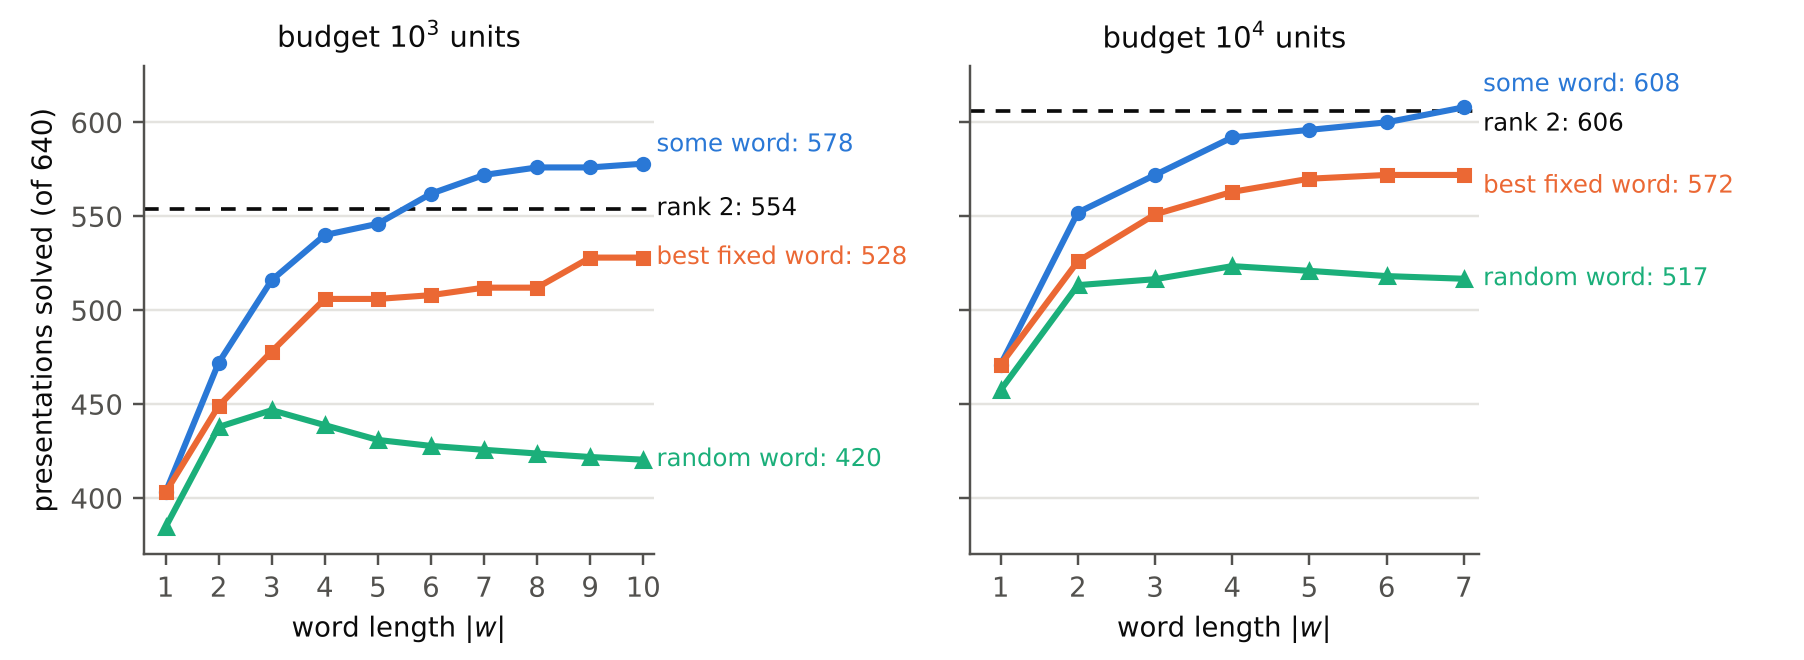
\includegraphics[width=\textwidth]{figures/stable_rank3_words.png}
\caption{Rank 3 against rank 2 on MS640. Some word and the best fixed word use the words of length at most $|w|$;
random word is $640$ times the share solved by the words of length exactly $|w|$. Dashed: rank 2.}
\label{fig:stable_words}
\end{figure}

\begin{table}[ht]
\centering
\small
\begin{tabular}{rrrrrrr}
\toprule
& & \multicolumn{2}{c}{words of length $|w|$} & \multicolumn{3}{c}{some word of length $\le|w|$}\\
\cmidrule(lr){3-4}\cmidrule(lr){5-7}
$|w|$ & words & solved & faster than rank 2 & solves & gained & lost\\
\midrule
1 & $2$ & $60.1\%$ & $0.0\%$ & $403$ & $0$ & $151$\\
2 & $6$ & $68.4\%$ & $1.1\%$ & $472$ & $0$ & $82$\\
3 & $18$ & $69.8\%$ & $0.6\%$ & $516$ & $0$ & $38$\\
4 & $54$ & $68.6\%$ & $1.1\%$ & $540$ & $4$ & $18$\\
5 & $162$ & $67.3\%$ & $0.9\%$ & $546$ & $8$ & $16$\\
6 & $486$ & $66.8\%$ & $0.7\%$ & $562$ & $16$ & $8$\\
7 & $1{,}458$ & $66.5\%$ & $0.6\%$ & $572$ & $20$ & $2$\\
8 & $4{,}374$ & $66.2\%$ & $0.6\%$ & $576$ & $22$ & $0$\\
9 & $13{,}122$ & $65.9\%$ & $0.5\%$ & $576$ & $22$ & $0$\\
10 & $39{,}366$ & $65.7\%$ & $0.5\%$ & $578$ & $24$ & $0$\\
\midrule
rank 2 & & $86.6\%$ & & $554$ & &\\
\bottomrule
\end{tabular}
\caption{Rank 3 at budget $10^3$. Solved: the share of the $640\times$words searches solved; faster: the share solved
in fewer units than rank 2, or solved where rank 2 fails. Gained: solved by some word, not by rank 2; lost: solved by
rank 2, by no word.}
\label{tab:stable_words}
\end{table}

\paragraph{Rank 3.} Rank 3 beats rank 2 only with the right word (Figure~\ref{fig:stable_words},
Table~\ref{tab:stable_words}). On the $554$ presentations rank 2 solves, a random word fails on $24.0\%$ and is
slower on $75.4\%$. The best fixed word, \texttt{yXYYYxyyy}, solves $528$. Some word passes rank 2 from length $6$
($578$ at length $10$; $608$ against $606$ at budget $10^4$), but finding it costs more than rank 2: trying the words
in shortlex order takes at least $41{,}711$ units on each of the $24$ gained, which rank 2 solves with $1{,}160$ to
$26{,}838$.

\paragraph{Why one letter costs more than one move.} With $w=x$, the relator $z^{-1}x$ lets one S-move turn a letter
$x^{\pm1}$ of another relator into $z^{\pm1}$, or back, without changing $\lambda$: $ux\cdot x^{-1}z=uz$. A state with
$m$ letters $x^{\pm1}$ thus has up to $2^m$ copies of the same length, all the same state once $z$ is set to $x$, and
the greedy pops them before any longer state. Over the $1{,}280$ searches with $|w|=1$, $97.5\%$ of the pops repeat a
state already popped, up to $z=x$. Where rank 2 solves and rank 3 fails, the $10^3$ pops reach a median of $12$
different states, while rank 2 needs a median of $116$ pops.


\paragraph{Ranks 4 and 5.} More generators are worse on every count (Table~\ref{tab:stable_ranks},
Figure~\ref{fig:stable_split}). Where rank 2 needs under $10$ units, almost every start solves but with more units;
the harder the presentation for rank 2, the more starts fail within the budget, and each added generator makes more
of them fail.
